\chapter{Results}
\label{ch:results}

[TODO, highlight more the temporal aspects of this work]

I analyzed three daily networks, these are referred to below as network~1~($N=922$), network~2~($N=978$) and network~3~($N=922$), or $g_1$, $g_2$, and $g_3$. Each network is aggregated for ten hours (108~000 frames) starting at 8~a.m. and lasting until 6~p.m. I chose the 20.08.2016, 22.08.2016, and 24.08.2016, because at this point in time the hive also contained tagged foragers, thus older bees. At the same time young bees were added to the colony, see table~\ref{tab:networks} for details. The age distribution for each network is shown in figure~\ref{fig:ages}. The match value, according to equation~(\ref{eq:match}) between network 1 and 2 is 85\%~(833 bees), between network 2 and 3, it is 84\%~(823 bees) and between network 1 and 3, it is 78\%~(716 bees).

\begin{table}
\centering
\caption[Sampling period]{\textbf{Sampling period} Overview of the chosen day networks including the number of added bees and the time they were added to the hive.}
\vspace*{5mm}
\begin{tabularx}{\textwidth}{ccccccc}
\toprule
{} & 20.08.16 & 21.08.16 & 22.08.16 & 23.08.16 & 24.08.16 \\
\midrule
Network ID & 1 & - & 2 & - & 3 & \\
Number of added bees & 0 & 0 & 110 & 60 & 0 \\
Time added & - & - & 2~p.m. & 6~p.m. & - \\
\bottomrule
\end{tabularx}
\label{tab:networks}
\end{table}
\begin{table}[htbp]
\small
\centering
\caption[Global network properties]{\textbf{Global network properties} $N$ number of nodes, $L$ number of links, $D$ diameter, $\langle d_{\texttt{max}} \rangle$ average path length, $\langle d \rangle$ diameter, $C_\Delta$ global clustering coefficient, $\langle k \rangle$ average degree and $\langle s \rangle$ represents the average strength, as introduced in section~\ref{sec:definitions}.}
\label{tab:stats}
\vspace*{5mm}
\begin{tabular}{rccccccccc}
\toprule
{} &  $N$ &   $L$ &  $D$ &  $\langle d_{\texttt{max}} \rangle$ &  $\langle d \rangle$ &   $C_\Delta$ & $\langle k \rangle$ &  $\langle s \rangle$ \\
\midrule
Snapshot 1 & 922 & 291179 & 0.69 & 3 & 1.32 &  0.79 & 631.62 & 5680.17 \\
Random 1  & 922 & 291179 & 0.69 & 2 & 1.31 &  0.69 & 631.62 & - \\ \midrule
Snapshot 2 & 978 & 256066 & 0.54 & 3 & 1.46 &  0.72 & 523.65 & 3977.94 \\
Random 2  & 978 & 256066 & 0.54 & 2 & 1.46 &  0.54 & 523.65 & - \\ \midrule
Snapshot 3 & 922 & 259421 & 0.61 & 3 & 1.39 &  0.75 & 562.74 & 4205.99 \\
Random 3  & 922 & 259421 & 0.61 & 2 & 1.39 &  0.61 & 562.74 & - \\
\bottomrule
\end{tabular}
\end{table}

\begin{figure}[htb]
	\centering
	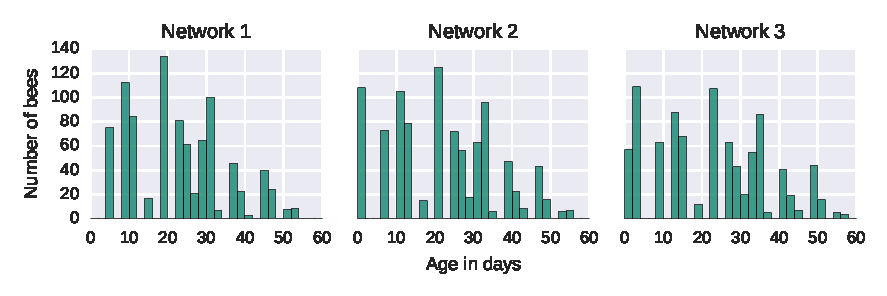
\includegraphics[width=1.0\textwidth]{Figures/ages}
	\caption[Age distribution per network]{\textbf{Age distribution per network} The width of a bar corresponds to two days. For each network bees with a negative age and the queen were removed (11, 10, and 9 bees).}
	\label{fig:ages}
\end{figure}


\section{Network Topology and Centrality}

Each network consists of one giant component. Table~\ref{tab:stats} summarizes basic network properties. The network density id for all networks over 50\%. The diameter is for all three networks $3$ and the average path length is below two. Compared to an Erdös-Renyi random graph the global clustering coefficient is higher, averaged over 100 runs per network with an SD below $0.00005$.

On average a bee is connected to 68\%, 54\% and 61\% percent of all bees in the network. Figure~\ref{fig:statDegreeDist} show a slighty bimodal degree distribution. The degree distribution does not follow a pow law, which is typical for real world social networks. 

The distribution of strength is shown in figure~\ref{fig:statStrengthDist} and the distribution of edge weights is depicted in figure~\ref{fig:statEdgeWeightDist}.

\begin{figure}[!t]
	\centering
	\begin{subfigure}[b]{1.0\textwidth}
	\centering
	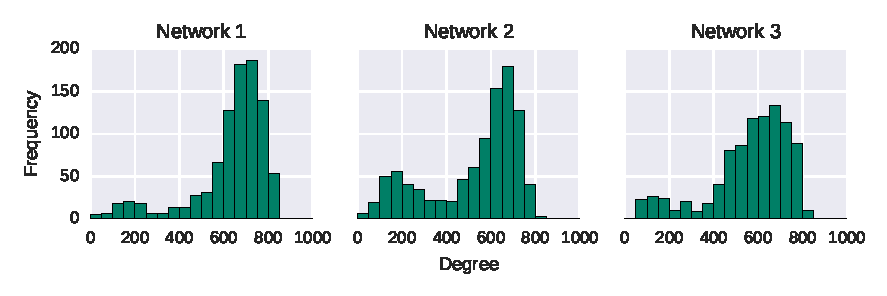
\includegraphics[width=0.92\textwidth]{Figures/stat-degreeDist}
	\caption[Degree distribution]{Degree distribution}
	\label{fig:statDegreeDist}
	\end{subfigure} 
	\begin{subfigure}[b]{1.0\textwidth}
	\centering
	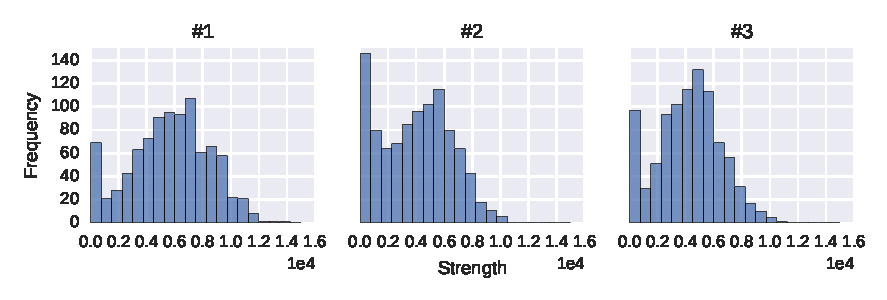
\includegraphics[width=0.92\textwidth]{Figures/stat-strengthDist}
	\caption[Strength distribution]{Strength distribution}
	\label{fig:statStrengthDist}
	\end{subfigure}
	\begin{subfigure}[b]{1.0\textwidth}
	\centering
	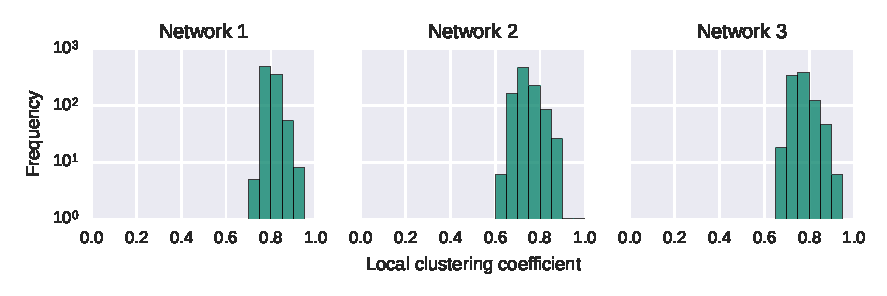
\includegraphics[width=0.92\textwidth]{Figures/stat-lccDist}
	\caption[Local clustering coefficient]{Local clustering coefficient}
	\label{fig:statlccDist}
	\end{subfigure}
	\begin{subfigure}[b]{1.0\textwidth}
	\centering
	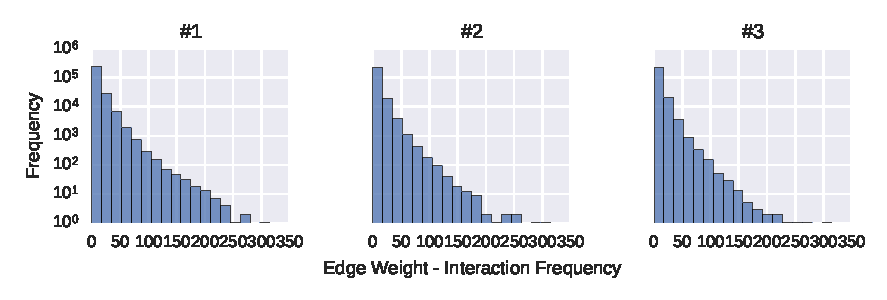
\includegraphics[width=0.92\textwidth]{Figures/stat-edgeWeightDist}
	\caption[Edge weight distribution]{Edge weight distribution}
	\label{fig:statEdgeWeightDist}
	\end{subfigure}
	\caption[Degree, strength and edge weight distribution]{\textbf{Degree, strength and edge weight distribution} for all three networks.}
	\label{fig:distributions}
\end{figure}


\begin{figure}[htb]
	\centering
	\begin{subfigure}[b]{1.0\textwidth}
	\centering
	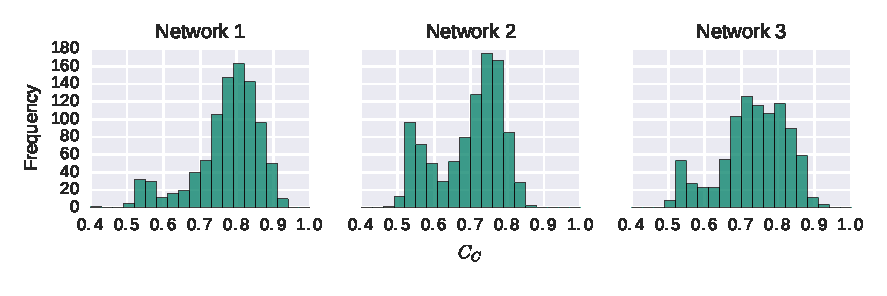
\includegraphics[width=0.92\textwidth]{Figures/stat-closenessDist}
	%\caption[Unweighted Closeness Centrality]{Unweighted Closeness Centrality}
	\label{fig:closenessDistUW}
	\end{subfigure} 
	\begin{subfigure}[b]{1.0\textwidth}
	\centering
	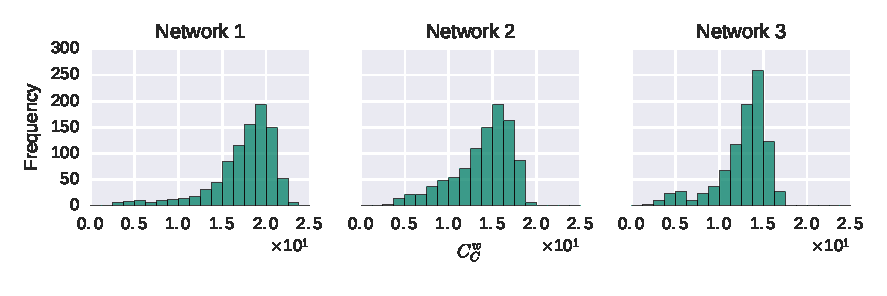
\includegraphics[width=0.92\textwidth]{Figures/stat-closenessWDist}
	%\caption[Weighted Closeness Centrality]{Weighted Closeness Centrality}
	\label{fig:closenessDistW}
	\end{subfigure}
	\caption[Closeness Centrality]{\textbf{Closeness Centrality}}
	\label{fig:closenessDist}
\end{figure}

\begin{figure}[htb]
	\centering
	\begin{subfigure}[b]{1.0\textwidth}
	\centering
	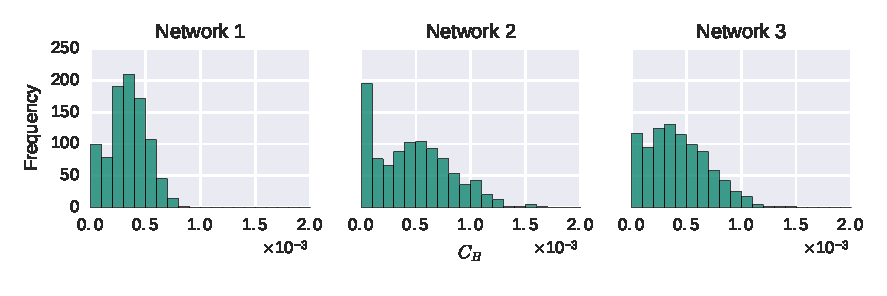
\includegraphics[width=0.92\textwidth]{Figures/stat-betweenDist}
	%\caption[Unweighted Closeness Centrality]{Unweighted Closeness Centrality}
	\label{fig:betweenDistUW}
	\end{subfigure} 
	\begin{subfigure}[b]{1.0\textwidth}
	\centering
	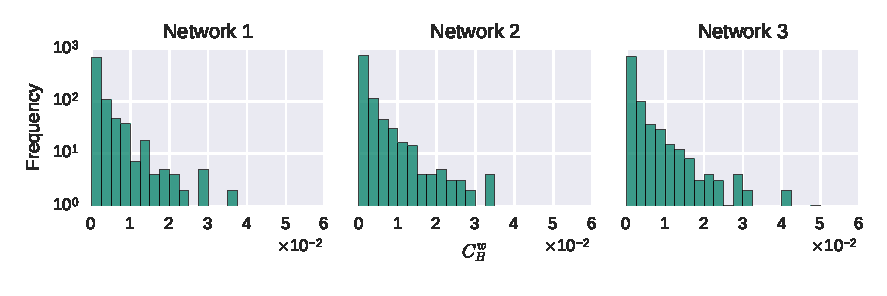
\includegraphics[width=0.92\textwidth]{Figures/stat-betweenWDist}
	%\caption[Weighted Closeness Centrality]{Weighted Closeness Centrality}
	\label{fig:betweenDistW}
	\end{subfigure}
	\caption[Betweenness Centrality]{\textbf{Betweenness Centrality}}
	\label{fig:betweenDist}
\end{figure}

\begin{figure}[htb]
	\centering
	\begin{subfigure}[b]{1.0\textwidth}
	\centering
	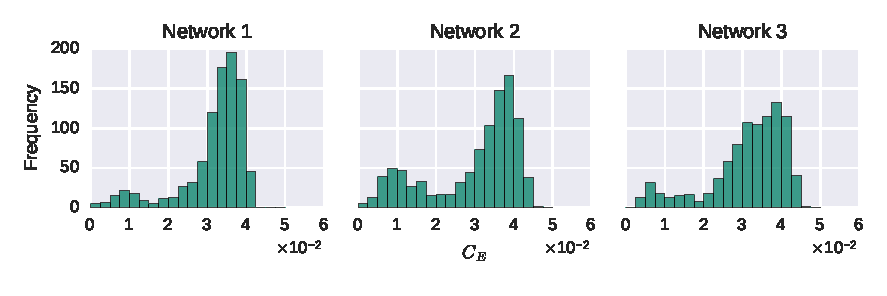
\includegraphics[width=0.92\textwidth]{Figures/stat-evcDist}
	%\caption[Unweighted Closeness Centrality]{Unweighted Closeness Centrality}
	\label{fig:betweenevcUW}
	\end{subfigure} 
	\begin{subfigure}[b]{1.0\textwidth}
	\centering
	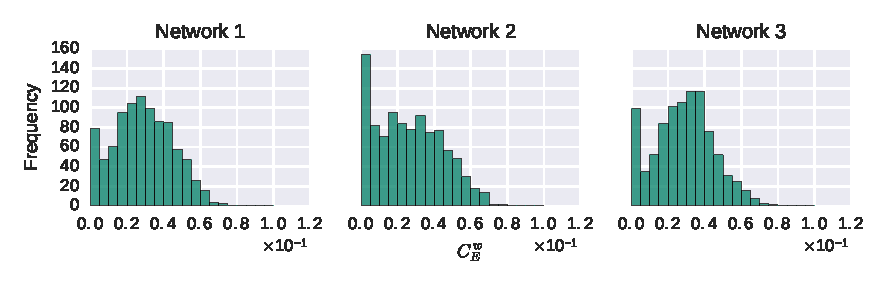
\includegraphics[width=0.92\textwidth]{Figures/stat-evcWDist}
	%\caption[Weighted Closeness Centrality]{Weighted Closeness Centrality}
	\label{fig:betweenevcW}
	\end{subfigure}
	\caption[Eigenvector Centrality]{\textbf{Eigenvector Centrality}}
	\label{fig:evcDist}
\end{figure}

\section{Node Level Metrics in Relation to the Age of Bees}

Closenes centrality (weighted and unweighted) in relation to age is depicted in figure~\ref{fig:closenessAge}. Betweennes centrality (weighted and unweighted) in relation to age is depicted in figure~\ref{fig:betweenAge}. Eigenvector centrality (weighted and unweighted) in relation to age is depicted in figure~\ref{fig:evcAge}.

\begin{figure}[htb]
	\centering
	\begin{subfigure}[b]{1.0\textwidth}
	\centering
	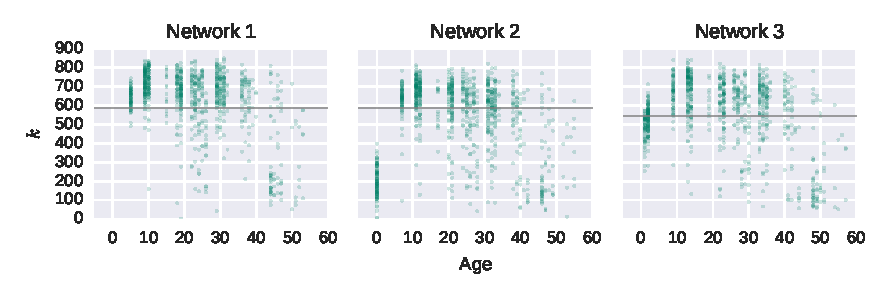
\includegraphics[width=0.92\textwidth]{Figures/stat-degreeAge}
	%\caption[Unweighted Closeness Centrality]{Unweighted Closeness Centrality}
	\label{fig:degreeAge}
	\end{subfigure} 
	\begin{subfigure}[b]{1.0\textwidth}
	\centering
	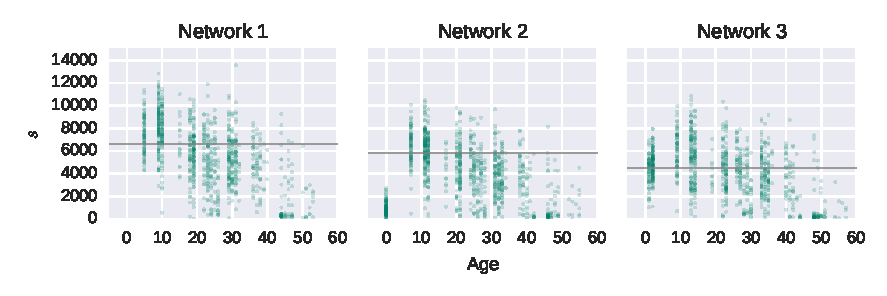
\includegraphics[width=0.92\textwidth]{Figures/stat-strengthAge}
	%\caption[Weighted Closeness Centrality]{Weighted Closeness Centrality}
	\label{fig:strengthAge}
	\end{subfigure}
	\begin{subfigure}[b]{1.0\textwidth}
	\centering
	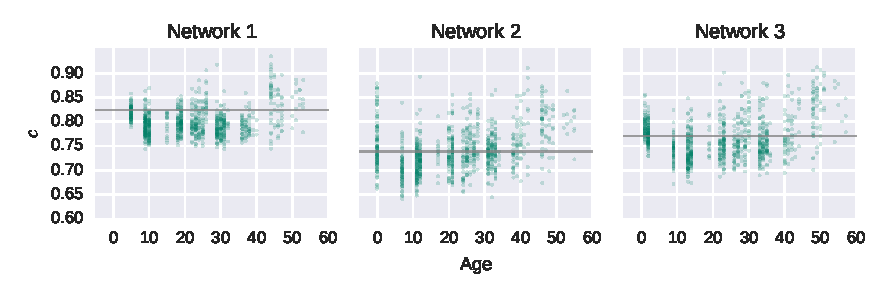
\includegraphics[width=0.92\textwidth]{Figures/stat-lccAge}
	%\caption[Weighted Closeness Centrality]{Weighted Closeness Centrality}
	\label{fig:lccsAge}
	\end{subfigure}
	\caption[Degree, strength and local clustering coefficient in relation to Age]{\textbf{Degree, strength and local clustering coefficient in relation to Age} The age is measured in days. The gray line corresponds to the quee. Bees with negative age are excluded.}
	\label{fig:degstrlcc}
\end{figure}

\begin{figure}[htb]
	\centering
	\begin{subfigure}[b]{1.0\textwidth}
	\centering
	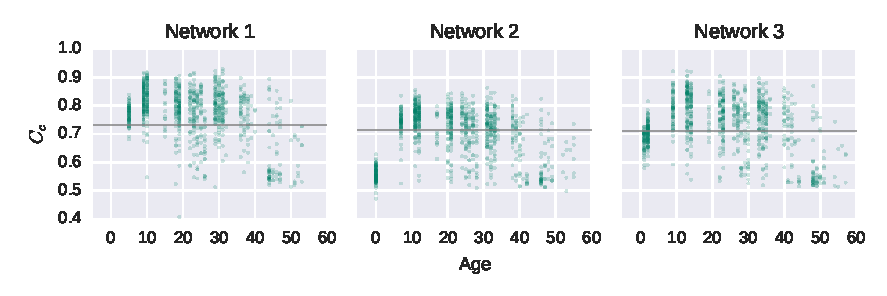
\includegraphics[width=0.92\textwidth]{Figures/stat-closenessAge}
	%\caption[Unweighted Closeness Centrality]{Unweighted Closeness Centrality}
	\label{fig:closenessAgeUW}
	\end{subfigure} 
	\begin{subfigure}[b]{1.0\textwidth}
	\centering
	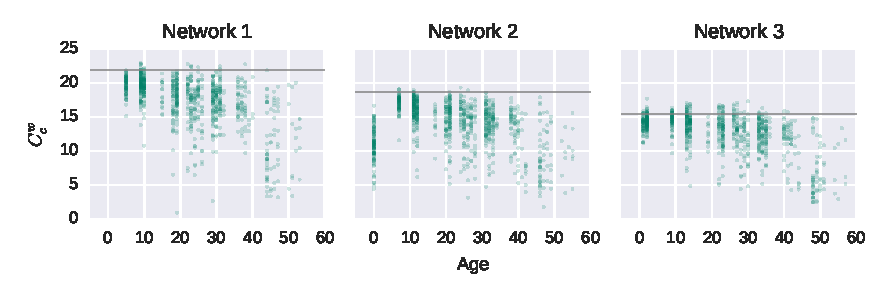
\includegraphics[width=0.92\textwidth]{Figures/stat-closenessWAge}
	%\caption[Weighted Closeness Centrality]{Weighted Closeness Centrality}
	\label{fig:closenessAgeW}
	\end{subfigure}
	\caption[Closeness Centrality and Age]{\textbf{Closeness Centrality and Age} The age is measured in days. The gray line corresponds to the quee. Bees with negative age are excluded.}
	\label{fig:closenessAge}
\end{figure}

\begin{figure}[htb]
	\centering
	\begin{subfigure}[b]{1.0\textwidth}
	\centering
	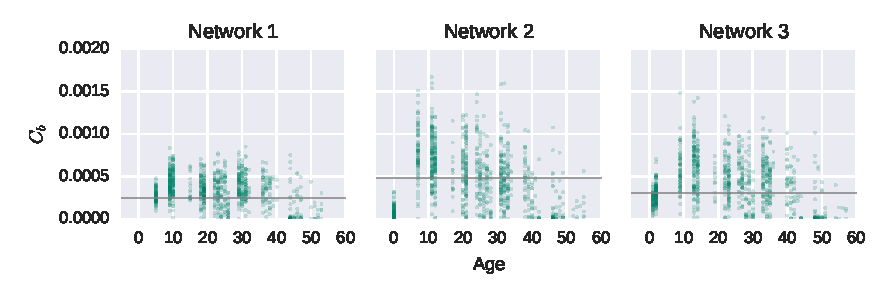
\includegraphics[width=0.92\textwidth]{Figures/stat-betweenAge}
	%\caption[Unweighted Betweennes Centrality]{Unweighted Betweennes Centrality}
	\label{fig:betweenAgeUW}
	\end{subfigure} 
	\begin{subfigure}[b]{1.0\textwidth}
	\centering
	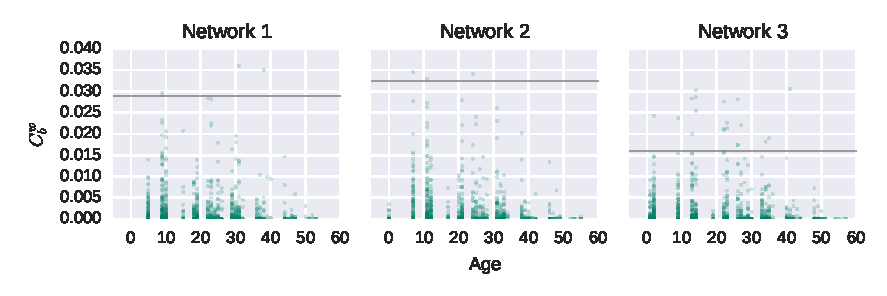
\includegraphics[width=0.92\textwidth]{Figures/stat-betweenWAge}
	%\caption[Weighted Betweennes Centrality]{Weighted Betweennes Centrality}
	\label{fig:betweenAgeW}
	\end{subfigure}
	\caption[Betweennes Centrality and Age]{\textbf{Betweennes Centrality and Age} The age is measured in days. The gray line corresponds to the quee. Bees with negative age are excluded.}
	\label{fig:betweenAge}
\end{figure}

\begin{figure}[htb]
	\centering
	\begin{subfigure}[b]{1.0\textwidth}
	\centering
	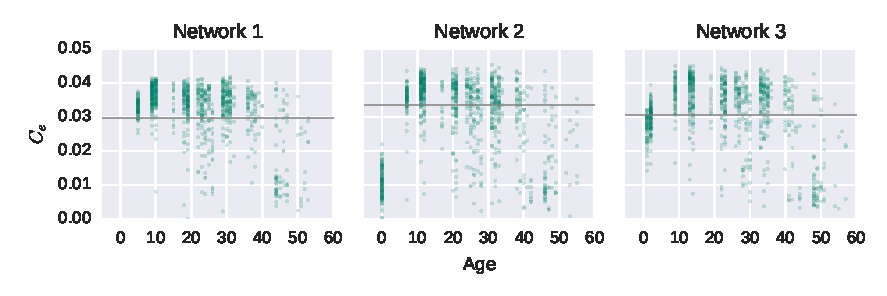
\includegraphics[width=0.92\textwidth]{Figures/stat-evcAge}
	%\caption[Unweighted Betweennes Centrality]{Unweighted Betweennes Centrality}
	\label{fig:evcAgeUW}
	\end{subfigure} 
	\begin{subfigure}[b]{1.0\textwidth}
	\centering
	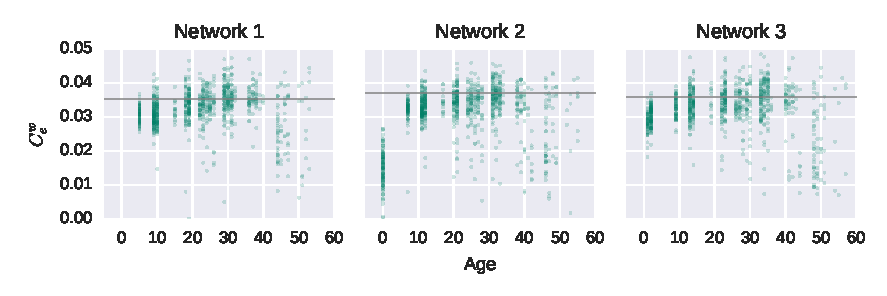
\includegraphics[width=0.92\textwidth]{Figures/stat-evcWAge}
	%\caption[Weighted Eigenvector Centrality]{Weighted Eigenvector Centrality}
	\label{fig:evcAgeW}
	\end{subfigure}
	\caption[Eigenvector Centrality and Age]{\textbf{Eigenvector Centrality and Age} The age is measured in days. The gray line corresponds to the quee. Bees with negative age are excluded.}
	\label{fig:evcAge}
\end{figure}

\clearpage
\section{Community Detection}

Using the leading eigenvector (LE) algorithm in all three networks two communities with about the same number of nodes are detected. With walktrap in network 1 two communities and in network 2 and 3, three communities. The exact number of community members for algorithm is shown in table~\ref{tab:networks}.

\subsection{Age Distribution of Communities}
The first community (LE-C1, WT-C1) contains the queen and bees who are on average younger than the second community (LE-C2, WT-C3). For walktraps third community it is a middle-aged community (WT-C2). The age difference for network 1 is $8.4$ days, for network 2 $10.9$ days, and for network 3 $14.4$ days on average for leading eigenvector communities.

The age distribution for each community and network is depicted in figure~\ref{fig:ageDistribution}.

A two sample Kolmogorov–Smirnov test showed, that for leading eigenvector communities, the age distributions are significantly different ($p< 0.001$). For walktrap C1 with C2 and C3 are significantly different, but C2 and C3 are not that much significant. Exact $p$-values are shown in table~\ref{tab:pvalues2}

\begin{table}
\centering
\caption[Overview about communities]{\textbf{Overview about communities per network} Communities marked with * contain the queen. Age and standard deviation (SD) are measured in days.}
\label{tab:communities}
\vspace*{5mm}
\begin{tabular}{lcrrrrr}
	\toprule
	{}  & ID & Members & Proportion & Age & SD\\
	\midrule
	\rowcolor{Gray}
	Leading eigenvector &&&&&\\
	\midrule 
	\quad Network 1  & C1 & $*434$  & 47.07\% & $16.81$ & $\pm17.91$ \\
	                 & C2 & $488$   & 52.93\% & $25.15$ & $\pm19.49$ \\
	\midrule   							
	\quad Network 2  & C1 & $*503$  & 51.43\% & $15.44$ & $\pm19.54$ \\
	                 & C2 & $475$   & 48.57\% & $26.37$ & $\pm18.01$ \\
	\midrule  
	\quad Network 3  & C1 & $*385$  & 41.76\% & $12.85$ & $\pm20.24$ \\
	                 & C2 & $537$   & 58.24\% & $27.26$ & $\pm17.84$ \\
    \midrule
    \rowcolor{Gray}
    Walktrap &&&&&\\
    \midrule 
	\quad Network 1 & C1 & $*431$ & 46.75\% & $16.76$ & $\pm17.92$\\
	                & C2 & $490$  & 53.15\% & $25.16$ & $\pm19.48$\\
	\midrule
	\quad Network 2 & C1 & $*372$ & 38.04\% & $12.98$ & $\pm19.00$\\
				    & C2 & $311$  & 31.80\% & $23.11$ & $\pm19.48$\\
				    & C3 & $294$  & 30.06\% & $28.15$ & $\pm16.77$\\            
	\midrule
	\quad Network 3 & C1 & $*231$  & 25.05\% & $7.09$  & $\pm19.60$\\
					& C2 & $301$  & 32.65\% & $23.83$ & $\pm17.22$\\
					& C3 & $390$  & 42.30\% & $27.63$ & $\pm18.48$\\
	\bottomrule
\end{tabular}
\end{table}

\begin{table}
\centering
\caption[Kolmogorov-Smirnov test]{\textbf{Kolmogorov-Smirnov test} $p$-values for leading eigenvector (LE) and walktrap (WT) for each network and its communities.}
\label{tab:pvalues2}
\vspace*{5mm}
\begin{tabular}{lcrrrrr}
	\toprule

	\rowcolor{Gray}
	 & & LE p-value & WT p-value\\
	\midrule 
	\quad Network 1  & C1, C2 & 5.1e-32 & 3.3e-31 \\
	\midrule   							
	\quad Network 2  & C1, C2 & 7.6e-38 & 2.3e-32 \\
					    & C1, C3 & & 1.3e-44\\
					    & C2, C3 & & 6.6e-05\\
	\midrule  
	\quad Network 3  & C1, C2 & 1.4e-64 & 1.8e-65\\
					    & C1, C3 & &3.9e-93\\
						& C2, C3 & &2.6e-05\\ 
	\bottomrule
\end{tabular}
\end{table}


\begin{figure}[htb]
	\centering
	\begin{subfigure}[b]{1.0\textwidth}
		\centering
		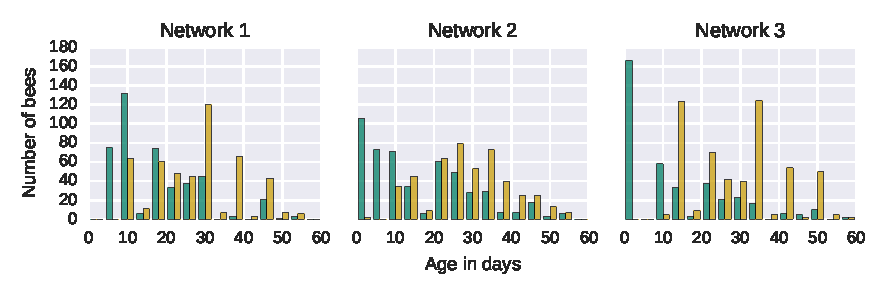
\includegraphics[width=1.0\textwidth]{Figures/ageDistribution-LE}
		\caption[Leading eigenvector]{Leading eigenvector}
		\label{fig:ageLE}
		\vspace*{5mm}
	\end{subfigure}
	%\vspace{1cm} 
	\begin{subfigure}[b]{1.0\textwidth}	
		\centering
		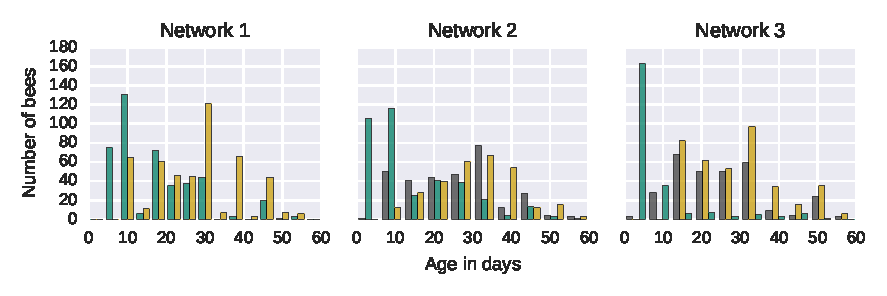
\includegraphics[width=1.0\textwidth]{Figures/ageDistribution-WT}
		\caption[Walktrap]{Walktrap}
		\label{fig:ageWT}
		\vspace*{5mm}
	\end{subfigure}
	%\vspace{1cm}
	\caption[Age distribution for each community and network] {\textbf{Age distribution for each community and network} The \emph{green} bar is the community containing the queen. The queens age is not included in the statistic. The \emph{orange} bars coresspond to the second community, containing older bees. The \emph{gray} bars is a third community only revealed by walktrap and contains middle-aged bees.}
	\label{fig:ageDistribution}
\end{figure}


\subsection{Spatial Distribution of Communities}
The two communities detected by leading eigenvector are located in two different regions of the honeycomb. The older community (\emph{orange} in figure~\ref{fig:communitiesPerNetworkLE})) is in all three networks closer to the hive exit and the younger community (\emph{green} in figure~\ref{fig:communitiesPerNetworkLE})) is situated in the comb center.
Walktrap revealed the same two communities like leading eigenvector for all three networks, with the same spatial distribution. For network 2 and 3, a third community (\emph{gray} in figure~\ref{fig:communitiesPerNetworkWT})) is located between the young and old community.

\begin{figure}[htb]
	\centering
	\begin{subfigure}[b]{1.0\textwidth}
		\centering
		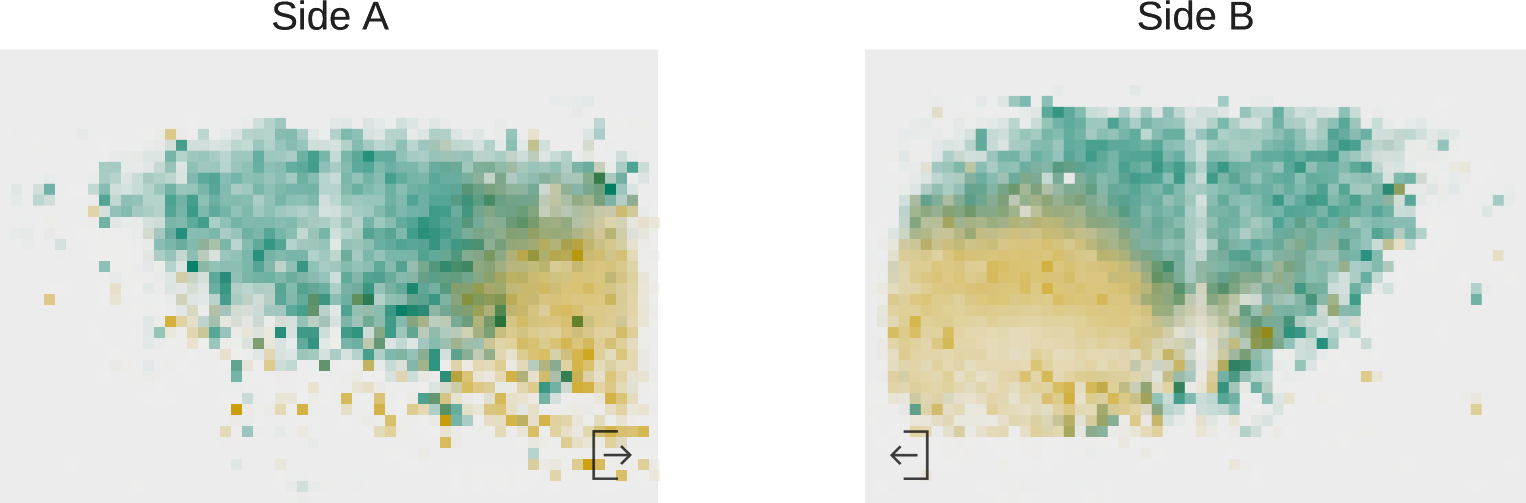
\includegraphics[width=\textwidth]{Figures/le_network1}
		\caption[Network 1]{Network 1}
		\label{fig:le1}
		\vspace*{5mm}
	\end{subfigure}
	%\vspace{1cm} 
	\begin{subfigure}[b]{1.0\textwidth}
		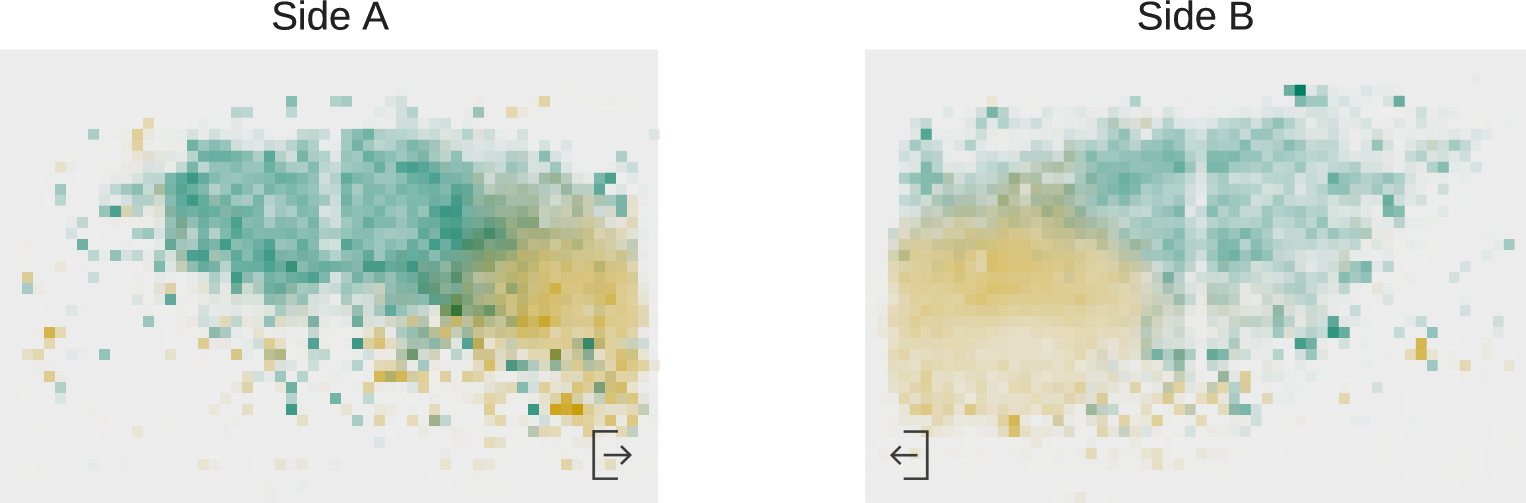
\includegraphics[width=\textwidth]{Figures/le_network2}
		\caption[Network 2]{Network 2}
		\label{fig:le2}
		\vspace*{5mm}
	\end{subfigure}
	%\vspace{1cm} 
	\begin{subfigure}[b]{1.0\textwidth}
		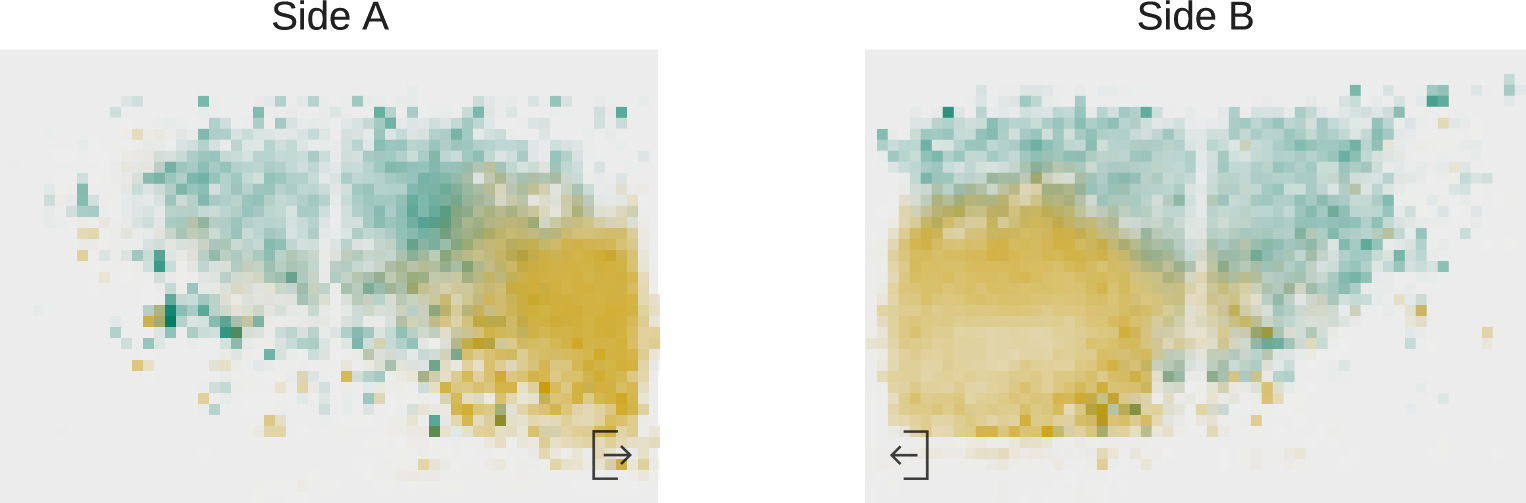
\includegraphics[width=\textwidth]{Figures/le_network3}
		\caption[Network 3]{Network 3}
		\label{fig:le3}
		\vspace*{5mm}
	\end{subfigure}
	\caption[Communities per network - leading eigenvector]{\textbf{Communities per network - leading eigenvector} The \emph{green} colour represents the younger community, containing the queen. The \emph{orange} color represents the older community. The hive exit on side A is on the bottom right and on side B on the bottom left. The data is aggredated for the complete timeframe of ten hours.}
	\label{fig:communitiesPerNetworkLE}
\end{figure}

\begin{figure}[htb]
	\centering
	\begin{subfigure}[b]{1.0\textwidth}
		\centering
		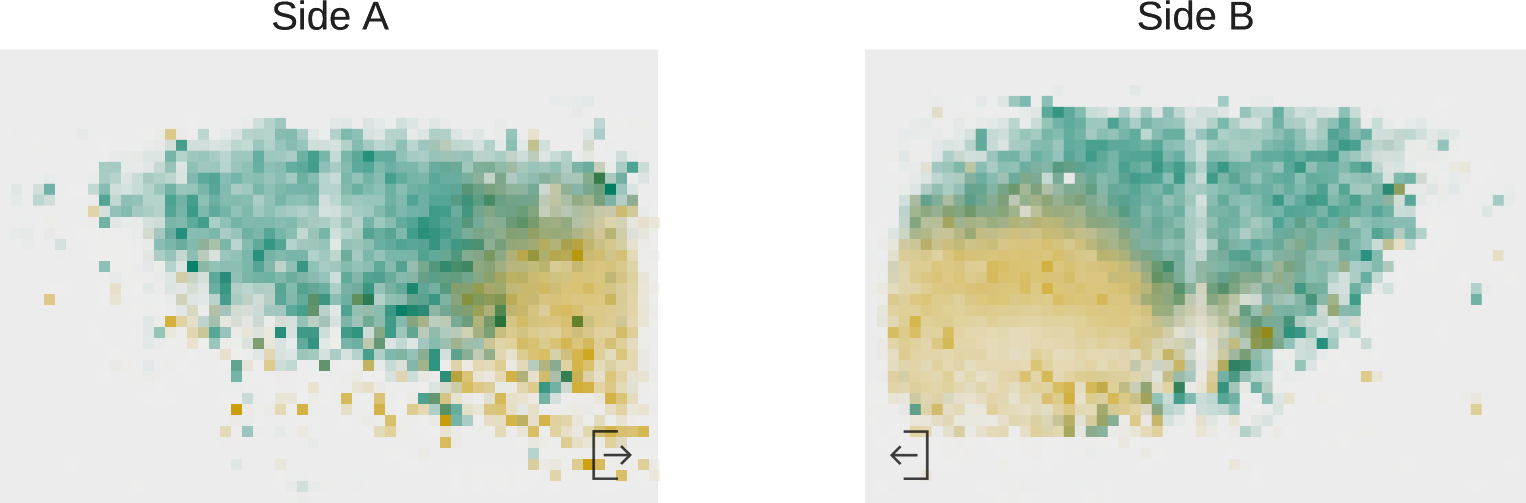
\includegraphics[width=\textwidth]{Figures/wt_network1}
		\caption[Network 1]{Network 1}
		\label{fig:wt1}
		\vspace*{5mm}
	\end{subfigure}
	%\vspace{1cm} 
	\begin{subfigure}[b]{1.0\textwidth}
		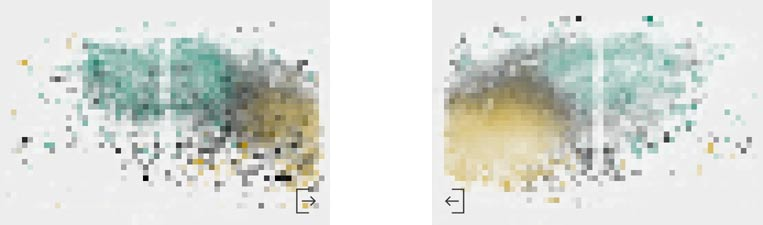
\includegraphics[width=\textwidth]{Figures/wt_network2}
		\caption[Network 2]{Network 2}
		\label{fig:wt2}
		\vspace*{5mm}
	\end{subfigure}
	%\vspace{1cm} 
	\begin{subfigure}[b]{1.0\textwidth}
		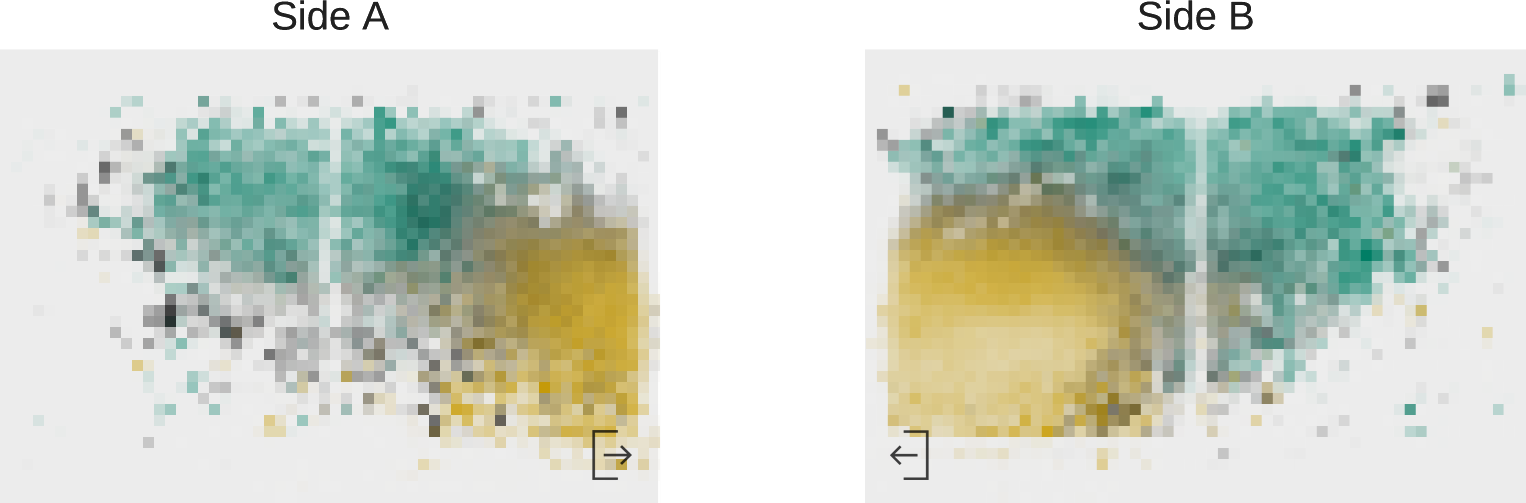
\includegraphics[width=\textwidth]{Figures/wt_network3}
		\caption[Network 3]{Network 3}
		\label{fig:wt3}
		\vspace*{5mm}
	\end{subfigure}
	\caption[Communities per network - walktrap]{\textbf{Communities per network - walktrap} The \emph{green} colour represents the younger community, containing the queen. The \emph{orange} color represents the older community. The \emph{gray} represents the middle-age community. The hive exit on side A is on the bottom right and on side B on the bottom left. The data is aggredated for the complete timeframe of ten hours.}
	\label{fig:communitiesPerNetworkWT}
\end{figure}

\clearpage

\section{Community members over time}
The match value between the two communities in successive time steps are calculated with formula~(\ref{eq:match}) and presented in figure~\ref{fig:membersLE} for the resulting communities using the leading eigenvector algorithm and figure~\ref{fig:membersWT} for the communities detected with walktrap.

\begin{figure}[htb]
	\centering
	\begin{subfigure}[b]{1.0\textwidth}
	\centering
	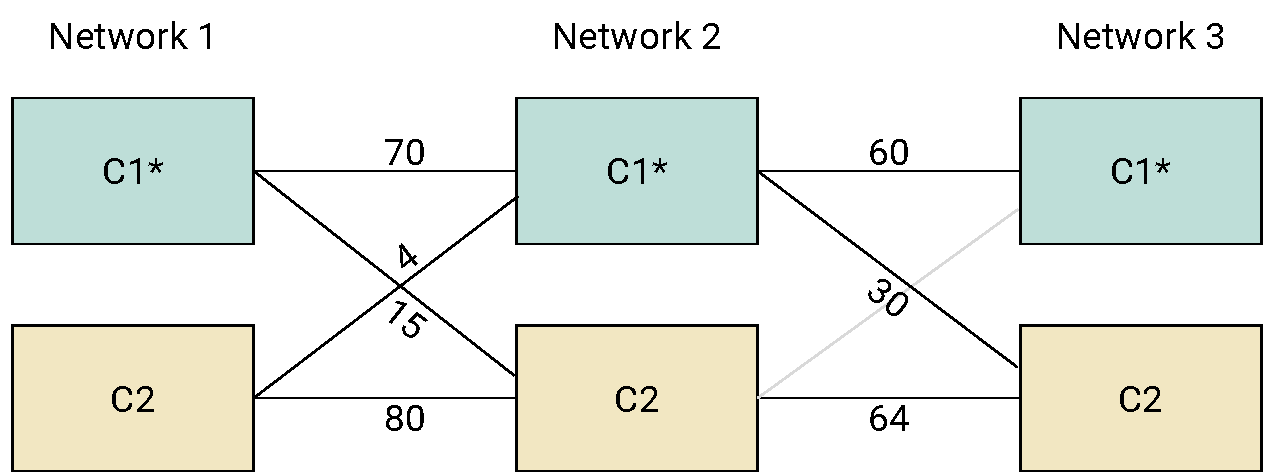
\includegraphics[width=.8\textwidth]{Figures/membersLE}
	\caption[Leading eigenvector communities]{Leading eigenvector communities}
	\label{fig:membersLE}
	\vspace*{5mm}
	\end{subfigure} 
	\begin{subfigure}[b]{1.0\textwidth}
	\centering
	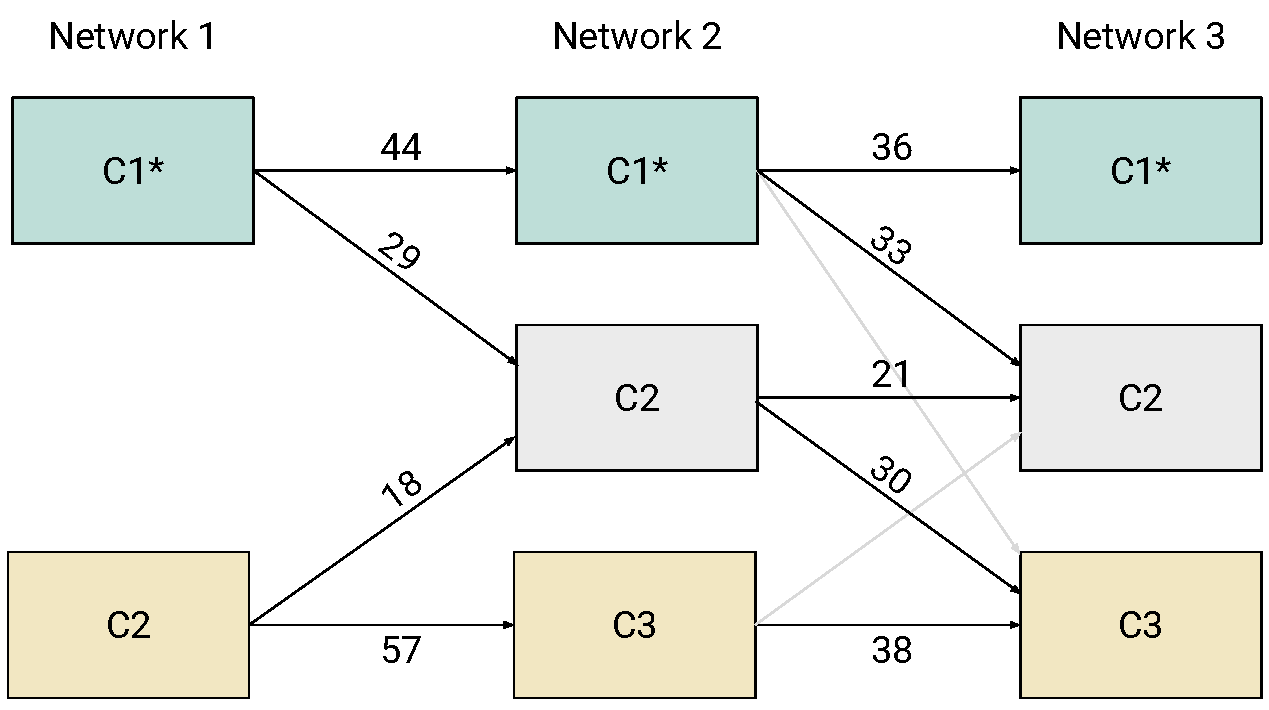
\includegraphics[width=.8\textwidth]{Figures/membersWT}
	\caption[Walktrap communities]{Walktrap communities}
	\label{fig:membersWT}
	\vspace*{5mm}
	\end{subfigure}
	\caption[Community matching]{\textbf{Community matching} The numbers indicate the match values in percent. The community marked with * contains the queen. \emph{Green} represents the younger community \emph{orange} the older community, and gray the middle-aged community. The light gray arrow represents match values below three percent.}
	\label{fig:members}
\end{figure}